\documentclass{standalone}

\usepackage[OT1]{fontenc}
\renewcommand*\familydefault{\sfdefault}
\usepackage{helvet,sfmath}
\usepackage{siunitx}

\usepackage{tikz}
\usetikzlibrary{arrows,calc,patterns}
\usepackage{tikz,tkz-euclide}

\definecolor{BlueDefault}{rgb}{0.2,0.2,0.7}

\begin{document}

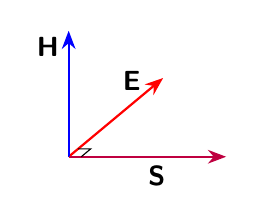
\begin{tikzpicture}[scale=0.4]
    \draw[-Stealth, thick, red] (0,0) to (3,2.5);
    \draw[-Stealth, thick, blue] (0,0) to (0,4);
    \draw[-Stealth, thick, purple] (0,0) to (5,0);
    \draw
    (0.4,0) to (0.7,0.25) to (0.3,0.25);
    \draw 
    (2.0,2.4) node{\(\mathbf{E}\)}
    (0,3.5) node[left]{\(\mathbf{H}\)}
    (2.8,0) node[below]{\(\mathbf{S}\)}
    ;
\end{tikzpicture}

\end{document}